\chapter{Implementation}

\textsl{This chapter provides the functional requirements of the application, explains the architecture of the developed research platform and presents some meaningful results and some steps forwards.}

\section{Functional Requirements}

\begin{figure}[h!]
	\centering
	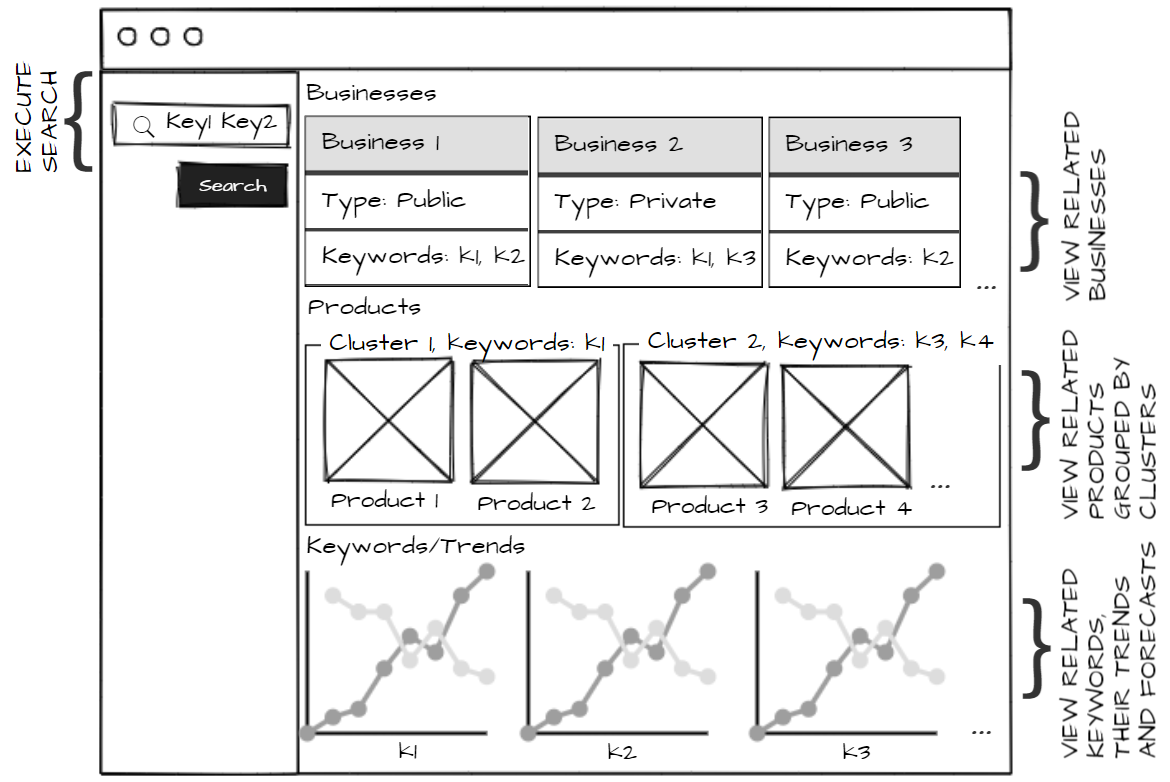
\includegraphics[scale=0.68]{img/wireframe.png}
	\caption{This wireframe shows the essential functionality of the implemented MRS.}
	\label{Implementation:Wireframe}
\end{figure}

\newpage
Functional requirements define the system behaviour and explain how the system responds to inputs. The minimum requirements that have been implemented are shown in figure \ref{Implementation:Wireframe}. The \ac{MRS} allows an user to perform a search by proving a list of keywords. When the user presses the search button the browser infers the location and language of the user and makes a request to the back-end which starts gathering and processing the data relevant to the keywords that have been provided. When this operation is successful, the system shows the results to the user in a report. The user can view the keywords that are related to the ones he provided, he can see the related businesses and the related products. The system is able to calculate a list of clusters for the products. The user can see the trends associated with the found keywords and for each trends view the forecasts. 

\section{System Architecture}

\begin{figure}[H]
	\centering
	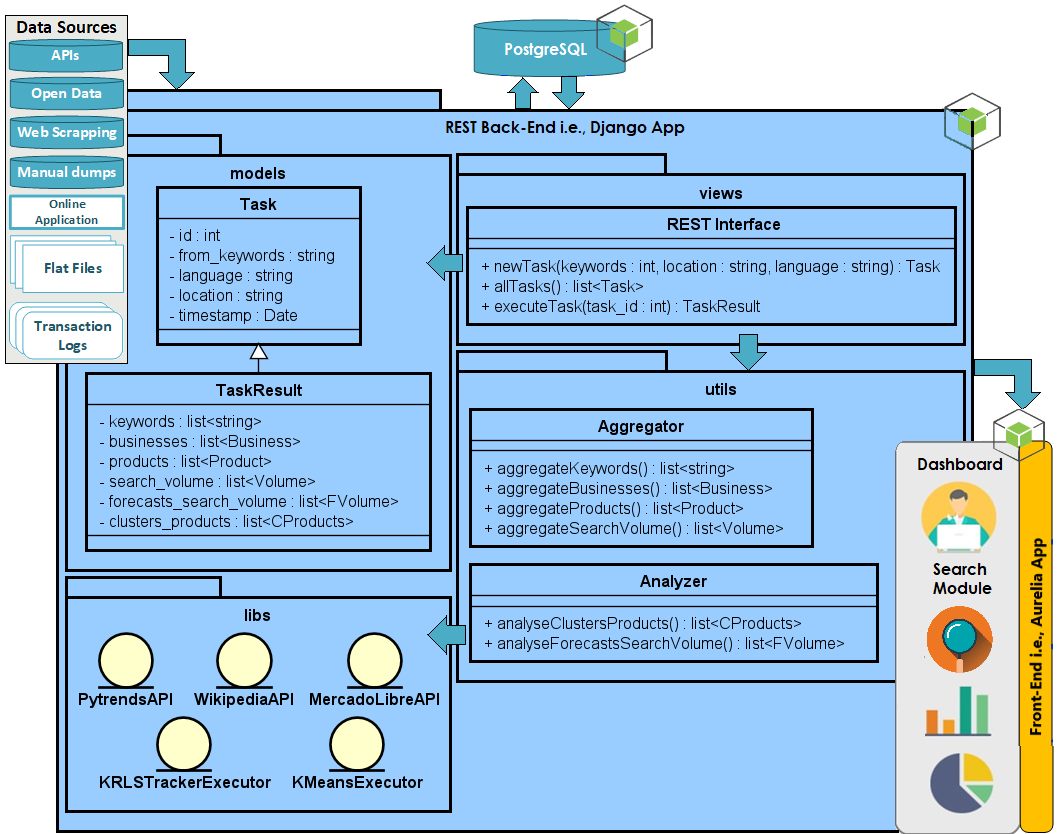
\includegraphics[scale=0.7]{img/architecture.png}
	\caption{This diagram contains the modules that implement the most recent version of the MRS.}
	\label{Implementation:System Architecture}
\end{figure} 

The \ac{MRS} is composed of a Back-End and a Front-End. The Back-End is served through Nginx and runs inside a Docker container. It is written using Django, a Python framework, and stores its data in a local PostgreSQL database. The main components of the server are the Aggregator and the Analyser. The Aggregator module uses various APIs and scraping objects to fetch data from the web and maps the collected information on a common model. In its current version, when an user performs a search, the system uses pytrends, a Python API that interacts with Google Trends, to generate 400 keywords and a time series with their interest over time. The interest over time trends come in the form of a value that goes from 0 to 100 and that is relative to the most searched term for a given location and time. Using the generated keywords the system fetches the info-boxes of businesses from Wikipedia and products information. The Analyser then takes care of analysing the data and performs regression and classification in order to extract useful marketing insights. The implemented market research platform can perform clustering on the products using k-means and do forecasting on trends using an online method known as Kernel Recursive Least Squares Tracker (KRLS-T). All this information is served to customers in JSON format through a REST interface. The Front End application was built using Aurelia, a JavaScript framework, and allows the users to use the functions of the \ac{MRS} and consume any marketing information through lists, graphs and tables. The products, businesses and related keywords are appropriately shown in a web browser with a design similar to figure \ref{Implementation:Wireframe}.

\newpage
\section{Forecasting using KRLS methods}


When a user performs a search the \ac{MRS} looks for a list of keywords associated with the keywords provided by the user and for every keywords is able to download a 5 years time series of trends that have a value that goes from 0 to 100 and that is relative to the most searched term on the Google search engine for a given location and time. The system then applies \ac{KRLS} regression to each 5 years time series set to perform forecasting and derives the values of these trends 2 years into the future. Before giving it as input to the algorithm every time series is prepared by mapping the dates to a 10 dimensional array of random values where the time positioning is achieved by shifting every row by one for every successive date. Algorithm \ref{Implementation:KRLS-T executor} shows this process more in detail.

\begin{algorithm}
	\caption{KRLS Tracker (KRLS-T) executor}
	\label{Implementation:KRLS-T executor}
	\begin{algorithmic}
		\STATE Fetch time series of keywords
		\STATE \(\lambda\) = forgetting factor
		\STATE c = regularization
		\STATE M = dictionary size
		\FOR{$i=1, 2, ...,M $}
		\STATE Consider \(dates_{i}\) and \(values_{i}\) of i-th keyword 
		\STATE Map every item of \(dates_i\) to a 10 dimensional vector \(dates_{i}^{'}\)
		\STATE forecasts i-th keyword are calculated with \(KRLST(dates_{i}^{'}, values_i, \lambda, c, M)\).
		\ENDFOR
	\end{algorithmic}
\end{algorithm}

\begin{figure}[h!]
	\centering
	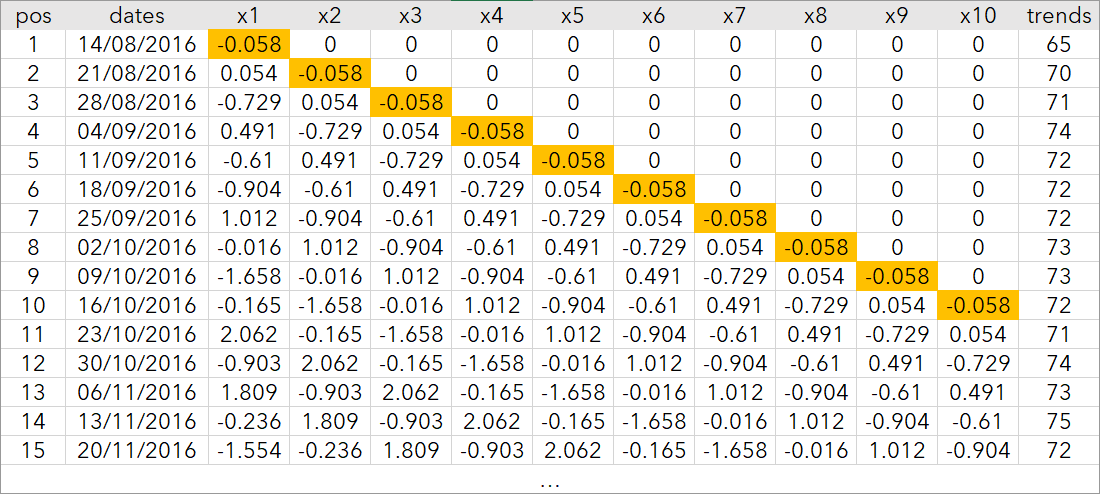
\includegraphics[scale=0.68]{img/datapreparation.png}
	\caption{This table shows how the dates of a time series are mapped to 10 dimensions filled with random values where time representation is obtained by shifting each successive date by one position.}
	\label{Implementation:Data Preparation}
\end{figure}

When the \ac{MRS} finishes calculating all the forecast the results are returned to the user which is able to visualize a time series for every keyword showing the actual demand and the forecasted demand. The interface the user sees looks very similar to figure \ref{Implementation:Keywords}.

\begin{figure}[h!]
	\centering
	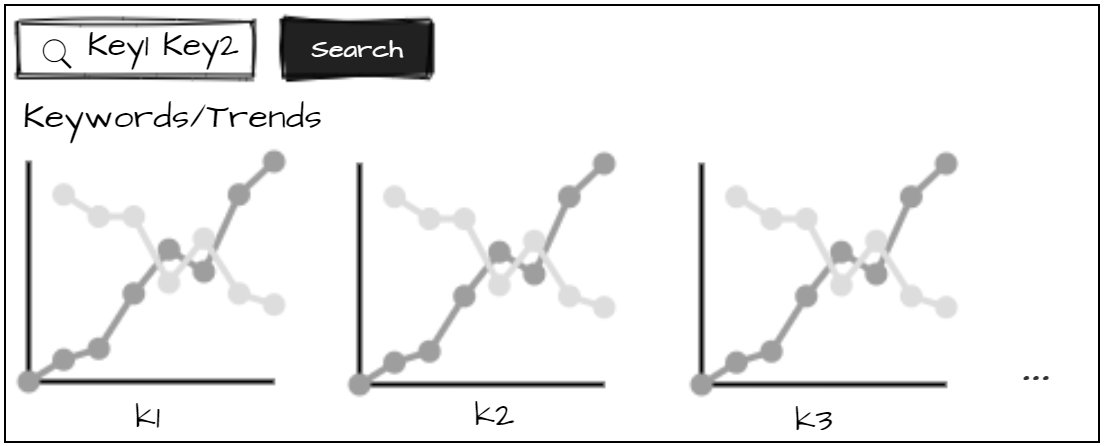
\includegraphics[scale=0.68]{img/keywords.png}
	\caption{This wireframe shows how the system displays the demand for each keyword.}
	\label{Implementation:Keywords}
\end{figure}

Marketing data is non-stationary which means that it is affected by several implicit variables. The goal of the current section is to show that \ac{KRLS} regression techniques are able to model such data and perform forecasting accurately. In order to understand which \ac{KRLS} variant is the most accurate, the algorithm was tested with different parameters and the corresponding \ac{MSE}s were calculated. The \ac{MSE}s have been calculated using a training set of 200 points and a test set of 60 points. Every time a new training point was added to the algorithm, the \ac{MSE} was calculated by subtracting the estimated values and the actual values of the test set. Only two kernel were used, the first being the radial basis function that has the following form:
\[K(X_i, X_j) = \exp(-\frac{\mid\mid X_i - X_j \mid\mid^2}{2\sigma^2})\]
The second is the a rational quadratic function that has the form:
\[K(X_i, X_j) = (1+\frac{\mid\mid X_i - X_j \mid\mid^2}{2\alpha l^2})^{-\alpha}\] 
When the algorithm uses no forgetting factor it means that it gives equal importance to all the training data that is available to it. On the contrary, the algorithm uses some weights for each base. The dictionary size drives how much of the data is kept as the basis of the algorithm. The data used for analysis is the demand relative to the keyword food.  


\begin{figure}[H]
	\centering
	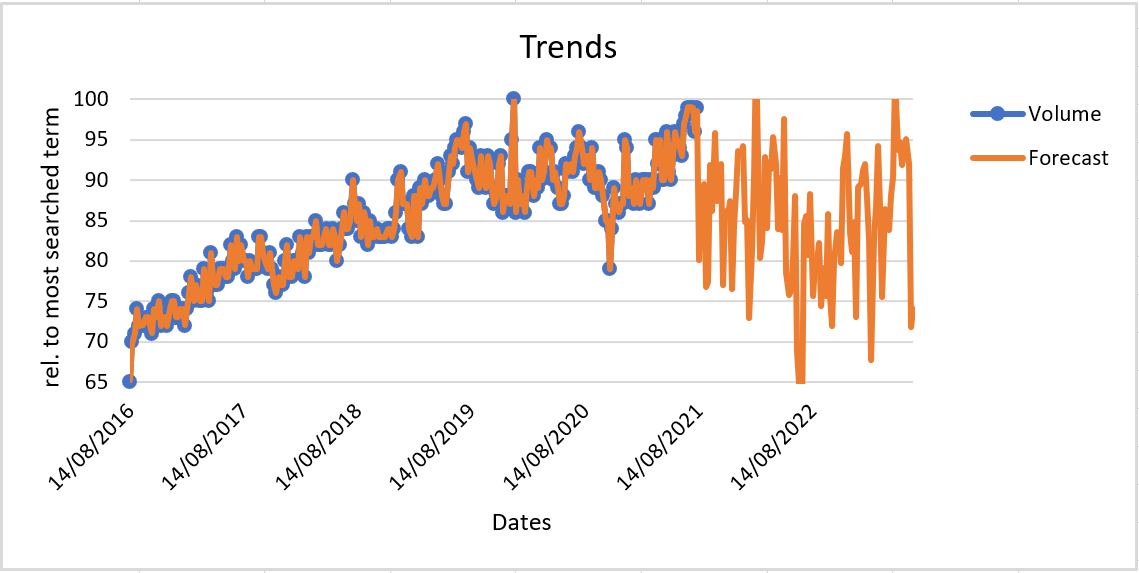
\includegraphics[scale=0.6]{img/exp1.png}
	\caption{The figure shows the search indexes over time relative to the keyword 'food' together with the estimated indexes calculated with a KRLS-T regressor that uses a RBF(2) kernel, a forgetting factor of 1, a regularization of 1e-4 and a dictionary size of 300 elements.}
	\label{Implementation:Trends 1}
\end{figure} 

\begin{figure}[H]
	\centering
	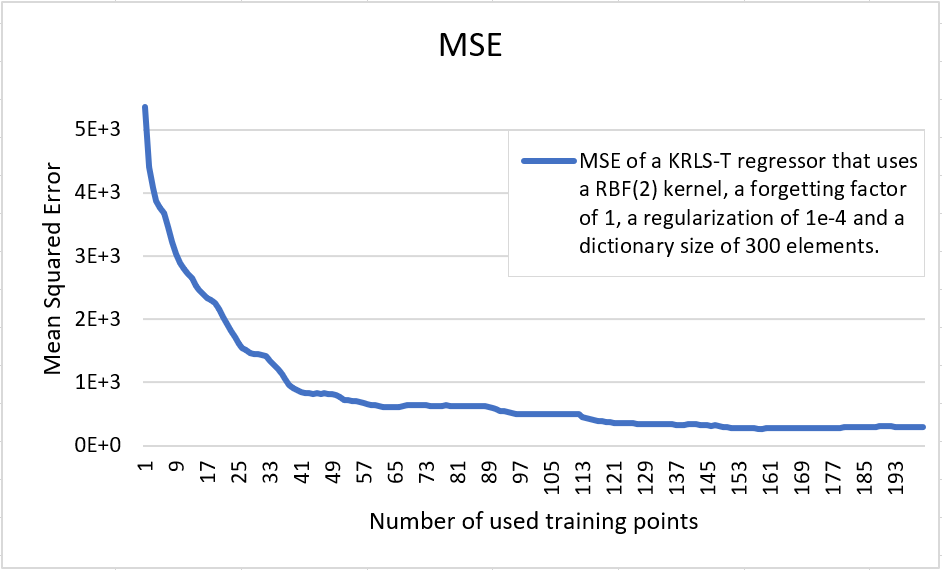
\includegraphics[scale=0.7]{img/exp1_mse.png}
	\caption{The figure shows the improvement over time of the Mean Squared Error of a KRLS-T regressor that models the demand of the keyword 'food' and uses a RBF(2) kernel, a forgetting factor of 1, a regularization of 1e-4 and a dictionary size of 300 elements.}
	\label{Implementation:MSE 1}
\end{figure} 

 
The algorithm utilized in figure \ref{Implementation:Trends 1} uses a radial basis function kernel, a dictionary of 300 data points and no forgetting factor. The results show that the chosen kernel does not perform very well with the provided data. Figure \ref{Implementation:MSE 1} demonstrates that the algorithm becomes more and more accurate as more training data is used, however it eventually stops improving; the forecasts are not very good as they deviate from the expectation. 

\begin{figure}[H]
	\centering
	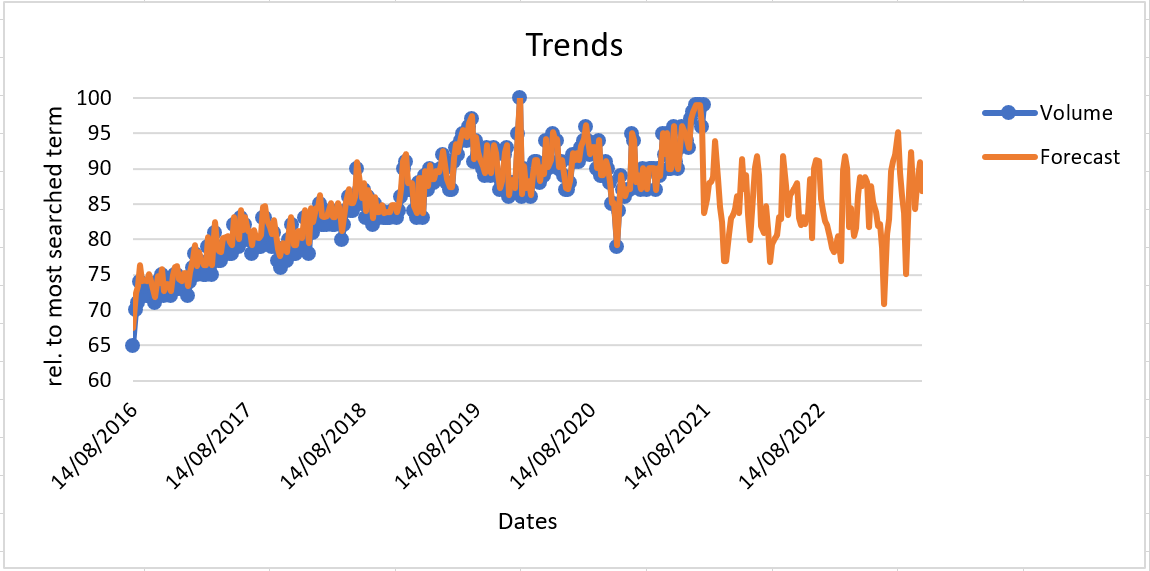
\includegraphics[scale=0.6]{img/exp2.png}
	\caption{The figure shows the search indexes over time relative to the keyword 'food' together with the estimated indexes calculated with a KRLS-T regressor that uses a RQ(2) kernel, a forgetting factor of 0.99999, a regularization of 1e-4 and a dictionary size of 300 elements.}
	\label{Implementation:Trends 2}
\end{figure} 

\begin{figure}[H]
	\centering
	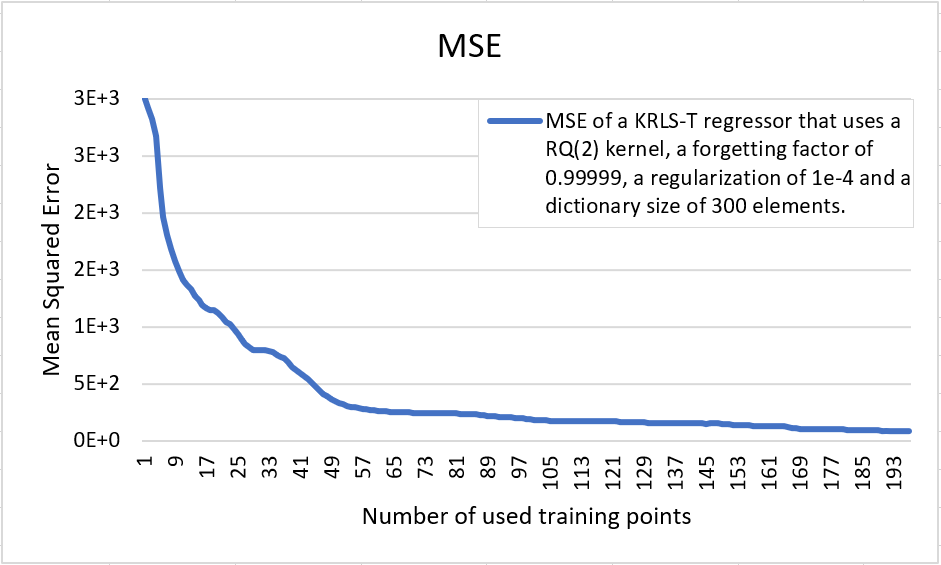
\includegraphics[scale=0.7]{img/exp2_mse.png}
	\caption{The figure shows the improvement over time of the Mean Squared Error of a KRLS-T regressor that models the demand of the keyword 'food' and uses a RQ(2) kernel, a forgetting factor of 0.99999, a regularization of 1e-4 and a dictionary size of 300 elements.}
	\label{Implementation:MSE 2}
\end{figure} 


The results shown in figure \ref{Implementation:Trends 2} have been calculated using a \ac{KRLS} regressor that employs a rational quadratic function, a dictionary of 300 elements and a back-to-prior forgetting factor of 0.99999. The performance appears much better than the previous case. The function does not approximate the data as well as before, but the forecasts are much closer to the expectation. Figure \ref{Implementation:MSE 2} demonstrates how the MSE gets much lower than the previous case and in general improves a lot faster with training without reaching a plateau. Because of the performance shown by this kernel it has been further tested with various other parameters.

\begin{figure}[H]
	\centering
	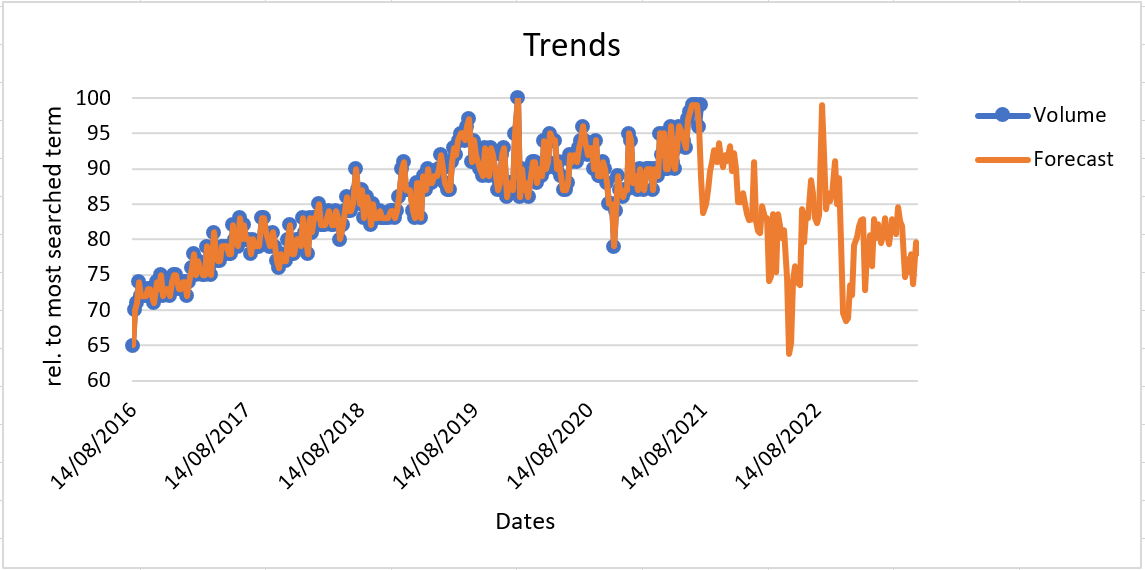
\includegraphics[scale=0.6]{img/exp3.png}
	\caption{The figure shows the search indexes over time relative to the keyword 'food' together with the estimated indexes calculated with a KRLS-T regressor that uses a RQ(2) kernel, a forgetting factor of 1, a regularization of 1e-4 and a dictionary size of 300 elements.}
	\label{Implementation:Trends 3}
\end{figure} 

\begin{figure}[H]
	\centering
	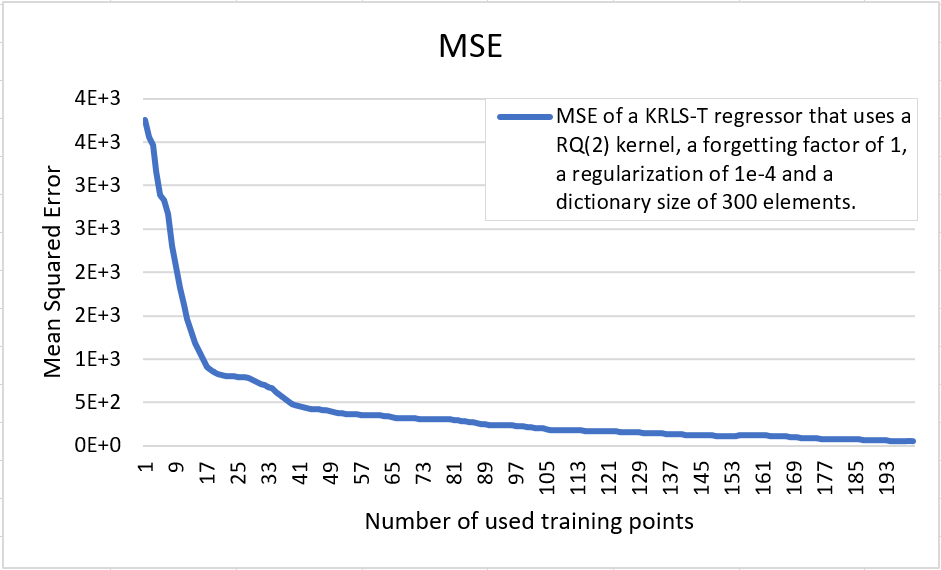
\includegraphics[scale=0.7]{img/exp3_mse.png}
	\caption{The figure shows the improvement over time of the Mean Squared Error of a KRLS-T regressor that models the demand of the keyword 'food' and uses a RQ(2) kernel, a forgetting factor of 1, a regularization of 1e-4 and a dictionary size of 300 elements.}
	\label{Implementation:MSE 3}
\end{figure} 

\newpage
The results displayed in figure \ref{Implementation:Trends 3} were calculated with a \ac{KRLS} regressor that employs a rational quadratic function, no forgetting factor and a dictionary of 300 elements. The performance appears to be similar to the previous case. The function can approximate the data as well as before, while the forecasts are slightly worse than the expected behaviour.

\begin{figure}[H]
	\centering
	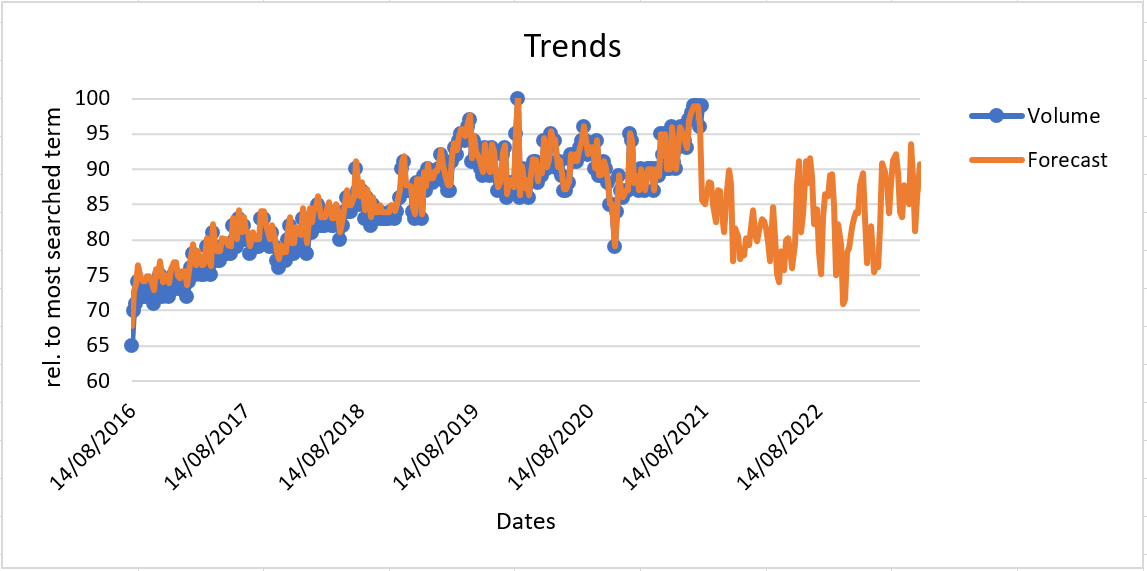
\includegraphics[scale=0.6]{img/exp4.png}
	\caption{The figure shows the search indexes over time relative to the keyword 'food' together with the estimated indexes calculated with a KRLS-T regressor that uses a RQ(2) kernel, a forgetting factor of 0.99999, a regularization of 1e-4 and a dictionary size of 100 elements.}
	\label{Implementation:Trends 4}
\end{figure} 

\begin{figure}[H]
	\centering
	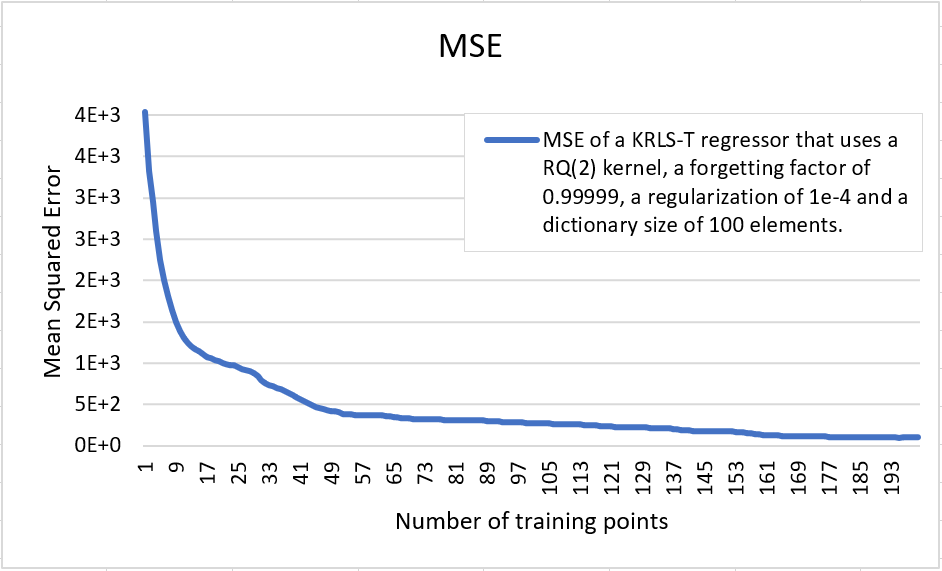
\includegraphics[scale=0.7]{img/exp4_mse.png}
	\caption{The figure shows the improvement over time of the Mean Squared Error of a KRLS-T regressor that models the demand of the keyword 'food' and uses a RQ(2) kernel, a forgetting factor of 0.99999, a regularization of 1e-4 and a dictionary size of 100 elements.}
	\label{Implementation:MSE 4}
\end{figure} 

\newpage
The results displayed in figure \ref{Implementation:Trends 4} have been calculated using a \ac{KRLS} regressor that employs a rational quadratic function and a back-to-prior forgetting factor of 0.99999, but a very small dictionary. The performance is apparently good but the forecasted values don't make much sense as can be seen in \ref{Implementation:MSE 4}. There is an abrupt drop at the intersection between the actual values and the estimated values.

\begin{figure}[H]
	\centering
	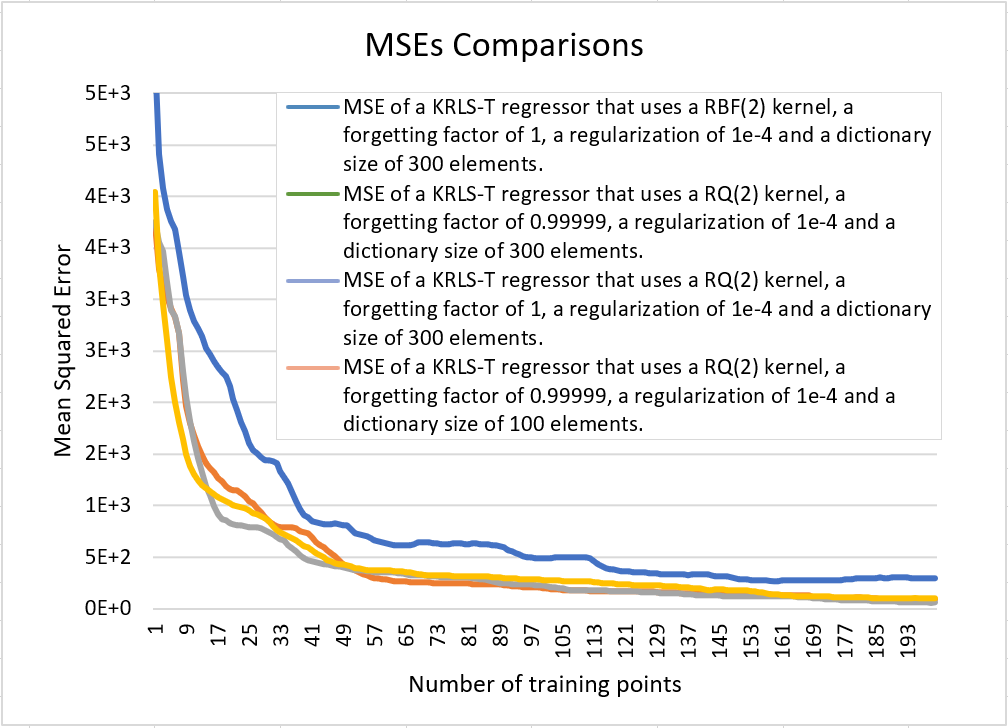
\includegraphics[scale=0.7]{img/mses.png}
	\caption{The figure shows a comparison between the MSEs obtained with different KRLS-T regressors that use different parameters. This MSEs are all relative to the modelling of the demand of the keyword 'food'.}
	\label{Implementation:MSEs}
\end{figure} 

As can be seen in figure \ref{Implementation:MSEs} the KRLS-T algorithm is more accurate when it uses a rational quadratic kernel. When using this type of kernel the performance is best when using no forgetting factor and a large dictionary size. However, even if the MSE appears better in this case, the actual forecasts appear much closer to the expectation when a back-to-prior forgetting factor is being used.

\newpage
\section{Clustering products using k-means}
The presented \ac{MRS} also implements a clustering method in which products are clustered into categories. Before fetching it to the algorithm, every product item is converted to a set of words and then again to a word frequency vector using the Python scikit-learn library TfidfVectorizer. After this operation it is possible to cluster the vectorized representation of the products into the Euclidean space with a k-means algorithm. The algorithm produces a list of clusters similar to figure \ref{Implementation:Clusters}.

\begin{figure}[h!]
	\centering
	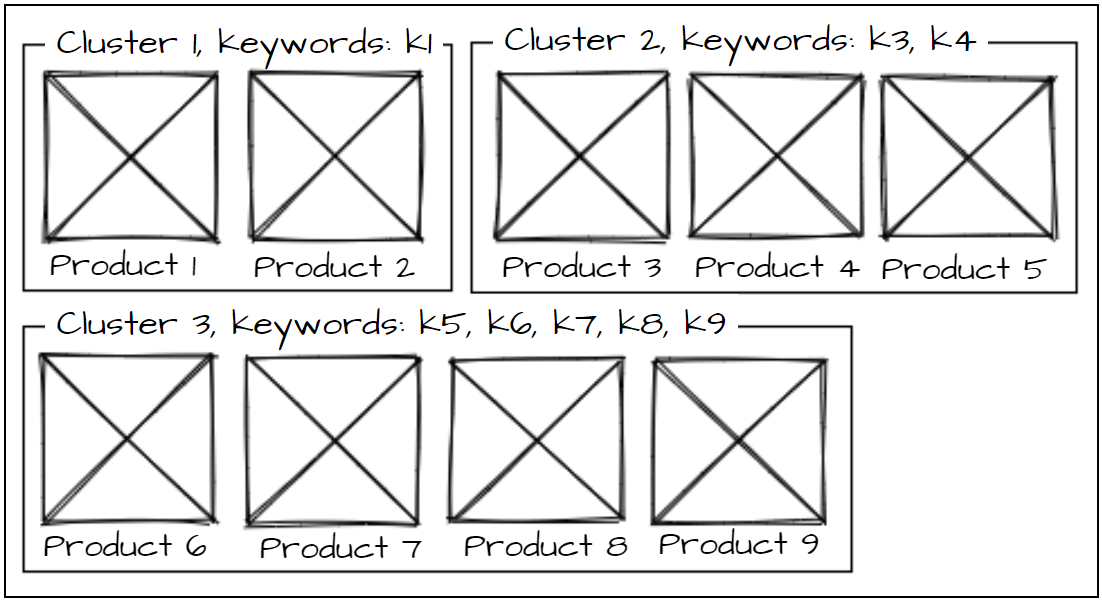
\includegraphics[scale=0.7]{img/clusters.png}
	\caption{This wireframe shows how products are placed inside clusters indexed by the set of the most common keywords within every cluster.}
	\label{Implementation:Clusters}
\end{figure}

In order to understand which is the optimal number of clusters k, the silhouette score is used, which is a value that measures how similar a point is to its own cluster compared to other clusters \cite{silhouette}. The Silhouette Value s(i) for each data point i is defined as follows: 

\[ 
\begin{sistema} 
s(i) = \frac{b(i) - a(i)}{\max (a(i), b(i))}, \mid C_{i} \mid > 1 \\ 
s(i) = 0, \mid C_{i} \mid = 1 
\end{sistema} 
\]
Where \(a(i) = \frac{1}{\mid C_{i} - 1 \mid} \sum\limits_{j \in C_{i}, i \neq j} \mid \mid i - j \mid \mid \) is the measure of similarity of the point i to its own cluster and \(b(i) = \min_{i \neq j} \frac{1}{\mid C_{i} \mid} \sum\limits_{j \in C_{i}} \mid \mid i - j \mid \mid \) is a measure of dissimilarity of i from points in other clusters. The optimal k is the value for which the Silhouette Score reaches its global maximum.


\begin{figure}[h!]
	\centering
	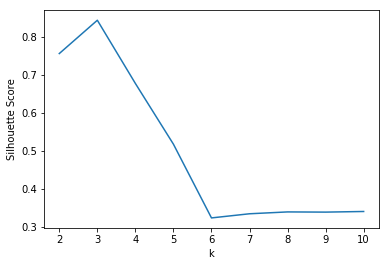
\includegraphics[scale=0.8]{img/silhouette.png}
	\caption{In an hypothetical scenario where the global maximum 3, the optimal number of clusters is also 3.}
	\label{Results:Silhouette Method}
\end{figure}

\newpage
\section{Future work}
It's possible to optimize the currently developed \ac{MRS}. In the current implementation the \ac{KRLS} regression performs forecasting on one time series at a time, but it's also possible to apply the \ac{KRLS} algorithms on all trends at once in a MIMO fashion. It is possible to make data gathering much faster by utilizing data sources that are local to the server rather than using remote data sources or scraping the web. It is also possible to improve the speed of data fetching by clustering data before the queries actually happen, so that the search system can simply look within the clusters relevant to the search. In general it is preferred to use data APIs than resort to web scraping and that is because the latter is very inefficient and sometimes it is not feasible, since websites change their DOM structure frequently and they might even change their DOM structure dynamically. This is why the current project uses a \ac{KRLS} scraper and not an Amazon or Ebay scraper. The \ac{MRS} can be made more general purpose by adding more research analytics.








